% !TEX root = thesis.tex

\chapter{Background}
\label{chapter:physics}
\thispagestyle{myheadings}

\graphicspath{{Physics/}}

\epigraph{If each energy quantum of the exciting light, independent of all others, emits its energy to electrons, the velocity distribution of the electrons will be independent of the intensity of the excitation light. On the other hand, the number of electrons leaving the body will be proportional to the intensity of the excitation light under otherwise similar circumstances.... It must therefore be assumed that the kinetic energy of an electron is used to generate many light energy quanta.}{\citet{einstein1905}}

The fine spatiotemporal dynamics of structured aurora have been studied for over a century, kicked off by leaders including Birkeland and Størmer from the 1890s onward.
Geoscientists by the time of \citet{birkeland1908} understood that particles flowing from the sun interacted with the geomagnetic field.
Before 1910 it was understood that perturbations of the geomagnetic field were directly related to the currents carried by what \citet{mcilwain1960} confirmed \textit{in situ} to be electrons for finely structured aurora.
A common metric for finely structured aurora is that aurora of width along $B_\perp$ one kilometer or less, which is associated with precipitating electrons.
The narrowest auroral structures driven by protons are nearly two orders of magnitude greater in width--interesting in their own right, but outside the scope of what the present HiST system is designed to observe.
Inverted-V and Alfvénic aurora are two well-known types of finely structured aurora with distinct electron acceleration mechanisms distinguishable by \textit{in situ}, radar and optical sensors.
Additional theories on fine structured auroral generation mechanisms include:
\begin{enumerate}
    \item Striped auroral patterns in diffuse background: whistler-mode upper band chorus \citep{nishiyama2012,sergienko2008}  
    \item ``smokelike'' aurora: consisting of multiple thin wispy legs of approximately \unit[1..5]{km} width \citep{ebihara2010}, thought to be an interchange instability between hot electrons disturbing cold plasma
\end{enumerate} 
While we have not specifically examined the latter two cases due to their relative rarity versus Alfvénic aurora, their characteristics are within the observational capabilities of the HiST system.

Geospace numerical modeling covers scales from particle-in-cell (PIC) simulations involving millions to billions of particles \citep{young2016} to the solar wind throughout the solar system \citep{echim2011}.
The lifecycle dynamics of a geomagnetic storm are modeled from the inner magnetosphere \citep{tsyganenko2005} out to the solar wind interface \citep{tsyganenko1996}.
While this dissertation focuses on the electron lifecycle in the ionosphere, sufficient understanding of the magnetosphere is a prerequisite for geospace study.
The \citet{johnson1960} model expressed in Figure~\ref{fig:1960mag} was rapidly improved upon in the next several years \citep{mead1964} with the benefit of an increasing number of \textit{in situ} measurements driving iteration of improved models and theories.
\begin{figure}
	\includegraphics[width=\linewidth]{gfx/1960mag}
	\caption{\citet{johnson1960} magnetospheric model, without benefit of \textit{in situ} measurements.}\label{fig:1960mag}
\end{figure}
In Figure~\ref{fig:1960mag}, the sun is far off the left side of the page.
In the absence of the roughly \unit[400]{km/s} solar wind, the nearly dipolar geomagnetic field would appear roughly symmetric about the magnetic equator and rotationally symmetric across all longitudes.

The solar wind compresses the dayside magnetic field, and drags out the magnetotail to tens of $R_E$.
Every several hours, a substorm occurs where the magnetotail to the right of Figure~\ref{fig:1960mag} becomes overloaded with plasma, a plasmoid detaches permanently, and the magnetotail settles in closer to Earth.
This cycle repeats endlessly, but with widely varying intensity of waves, particles, and ultimately precipitation incident into the ionosphere as represented in Figure~\ref{fig:magcirc}.
\begin{figure}\centering
	\includegraphics[width=\linewidth,trim=50 370 150 40,clip]{gfx/magcirc}
	\caption{Simplified model for two mechanisms responsible for structured aurora. 
		The parallel potential lines represent double-layers leading to inverted-V aurora. 
		The sinusoid represents IAW acceleration. 
		The contours represent $B$.}
	\label{fig:magcirc}
\end{figure}
Conservation laws dictate that the gradients involved in geomagnetic system reconfiguration must be felt throughout the geomagnetic system.
The magnetic field lines act as invisible transmission lines where ions and electrons travel freely, mirroring between the lower magnetosphere and magnetotail.
Particles that gain sufficient energy, whether via acceleration processes or other events are at risk of being lost into the ionosphere through stochastically predictable, TRANSCAR modeled energy deposition processes.
%The cold return current comes back up $B$ into the magnetosphere, closing the circuit depicted in Figure~\ref{fig:migcircuit}.
%\begin{figure}
%	\includegraphics[width=\columnwidth]{gfx/migcircuit}
%	\caption{Alfven-wave transmission of magnetosphere-ionopshere-ground coupling, from \citet{kikuchi2014}.}
%	\label{fig:migcircuit}
%\end{figure}
%\citet{kikuchi2014} further developed the circuit element model to compute characteristic impedance and reflection coefficients of the Alfvénic transmission line model and the waveguide model coupling ionosphere to ground.
%%\begin{figure}
%	\includegraphics[width=\linewidth]{../gfx/mi-transmission-line}
%	\caption{\citet{kikuchi2014} circuit element model to compute reflection coefficients for the Alfvenic M-I coupling interface and waveguide model for G-I coupling.}
%	\label{fig:distcirc}
%\end{figure}

These lost particles do not go quietly, rather their ``death'' is transmitted via electromagnetic waves from ELF through HF \citep{labelle2002}, as well as heat, light and X-rays \citep{raymont2008}.
Strictly speaking the particles are not lost, but they may join the cold plasma background, participate with the currents in the auroral electrojet and/or once again rejoin the current systems in the magnetosphere \citep{hargreavesbook}.
Although the understanding of auroral generation mechanisms are still incomplete at Earth and other planetary bodies, searches for radio \citep{nichols2012} and UV \citep{france2010} emissions from exoplanets have been undertaken.
Exoplanet auroral measurements help constrain the atmospheric morphologies and compositions.
Some of the challenges of quantifying auroral radio emissions in the tens of MHz range have been complicated by possibly interfering radio emissions from the magnetosphere of Jupiter \citep{labelle2002}, so more careful study is needed.
The many types of emissions emanating throughout the auroral lifecycle would consume volumes to describe, thus this chapter covers the topics necessary for elucidating the remainder of the dissertation.

This dissertation presents new ground-based observational capabilities associating ionospheric plasma flows and turbulence with Alfvén wave accelerated electron precipitation.
In this chapter physical context is provided for discussion in the following chapters concerning characterization of ionospheric turbulence associated with Alfvénic aurora.
One of the fundamental behaviors influencing the scale of aurora seen, and distinguishing between the behavior of electron aurora versus proton aurora is the gyration of charged particles in the presence of a magnetic field.
We therefore begin the physics background with single particle motion and describe the acceleration of these particles by Alfvén waves.
The energy deposition and production of auroral light emissions rounds out this chapter.

\section{Planetary Plasma}
Plasma about planetary bodies are infused with magnetic fields. 
For those planetary bodies without intrinsic magnetic fields, crustal magnetic fields such as at Mars and induced magnetic fields caused by the magnetic field lines draping around the planetary body nonetheless are essential to describing particle behavior.
Comets also experience an induced magnetosphere, as confirmed by \textit{in situ} measurements \citep{israelevich1994}.
Although diagrams of the geomagnetic system lend themselves to complexity, the basic particle behavior can be described starting with Newton's Second Law of Motion.


\FloatBarrier
\subsection{Single Particle Motion}
The basic equation of motion for a mass $m$ experiencing a force $\vect{F}$ is
\begin{equation}\label{eq:Feqma}
\vect{F}=m\vect{a} = m \frac{d\vect{v}}{dt}.
%\marginnote{eqn. of motion}
\end{equation}
In the presence of electric field $\vect{E}$, the Lorentz force on a particle with charge $q$ is
\begin{equation}\label{eq:lorentzforceBeq0}
\vect{F} = q\vect{E}.
%\marginnote{Lorentz force, \ensuremath{B\equiv0}}
\end{equation}
In the presence of a magnetic field $\vect{B}$ and electric field $\vect{E}$, a particle at rest will be accelerated and gyrate about $\vect{B}$, driven by the Lorentz force
\begin{equation}\label{eq:lorentzforce}
\vect{F} = q\left(\vect{E} + \vect{v}\times\vect{B}\right).
%\marginnote{Lorentz force}
\end{equation}
The decomposition of \eqref{eq:lorentzforce} into components
\begin{equation}\label{eq:Fperppar}
\vect{F} = \vect{F}_\parallel + \vect{F}_\perp
\end{equation}
where $\vect{F}_\parallel\in \vect{F} \parallel \vect{B}$ and $\vect{F}_\perp \in \vect{F} \perp \vect{B}$\ leads  to the notion that charged particles will gyrate in a magnetic field, with motion along $\vect{B}$ driven by $\vect{E}$ \citep{cravensbook}. 

For simplicity we drop the vector symbol where the context is clear.
The sign of $q$ indicates that positive and negative particles will move in opposite direction for both $F_\parallel$ and $F_\perp$. 
Aurora is observed \citep{borovsky1993} from the solution of~\eqref{eq:Feqma} for particles along $B$
\begin{equation}\label{eq:vpar}
v_\parallel = v_{\parallel,0} + \frac{F_\parallel}{m}t
%\marginnote{\ensuremath{v \parallel B}}.
\end{equation}
The gyroradius
\begin{equation}\label{eq:gyrad}
r_L = \frac{m_s v_\perp}{qB}
%\marginnote{gyroradius}
\end{equation}
and gyrofrequency
\begin{equation}\label{eq:gyfreq}
\Omega_s = \frac{q B}{m_s}
%\marginnote{gyrofrequency}
\end{equation}
follow from solving for 
\begin{equation}\label{eq:vperp}
v_\perp^2 = v_x^2 + v_y^2 
%\marginnote{\ensuremath{v \perp B}}
\end{equation}
with components
\begin{align}
v_x &= v_\perp \cos{\left( \Omega t + \theta \right)} \label{eq:vxy} \\
v_y &= \mp v_\perp \sin{\left( \Omega t + \theta \right)} \nonumber.
\end{align}
The pitch angle
\begin{equation}\label{eq:pitch}
\alpha_p = \tan^{-1}{\frac{v_\perp}{v_\parallel}}
%\marginnote{pitch angle}
\end{equation}
of a particle is the angle between $\vect{v}$ and $\vect{B}$.
As discussed in section~\ref{sec:losscone}, pitch angle is important for determining which particles are most likely to be lost during magnetic mirroring and thereby potentially appearing as aurora.
\FloatBarrier
\subsection{Magnetic Mirroring}\label{sec:mirror}
In general, geomagnetic field lines are not straight. 
The geomagnetic field $B$ converges near Earth and in the magnetotail. 
A significant percentage of the ions and electrons trapped in the geomagnetic field ``mirror''.
Magnetic mirroring here means that $v_\parallel$ changes sign, reversing the direction of particle travel along $B_\parallel$ in the lower magnetosphere and in the magnetotail. 
If via external fields or system reconfiguration a particle's $v_\parallel$ grows significantly enough relative to $v_\perp$, that is, the particle pitch angle \eqref{eq:pitch} decreases, the particle will enter the loss cone and penetrate into the ionosphere.

For a collisionless plasma with slowly changing fields, that is, where the scales of field gradients are small compared to the particle gyroradius, the magnetic moment of the particle \citep{kivelson,chenbook}
\begin{equation}\label{eq:adiabatic1}
\mu = \frac{ m v^2_\perp}{2B}
\end{equation}
remains constant.
When the direction and magnitude of $B$ and $v_\perp$ in \eqref{eq:adiabatic1} change slowly, $\mu$ is the constant known as the first adiabatic invariant. 
Converging $B$-field lines imply $B$ is increasing. 
Since particle mass $m$ is a constant and $\mu$ must remain approximately constant, $v_\perp$ must increase so that $\frac{v^2_\perp}{B}$ remains constant while maintaining a constant
\begin{equation}\label{eq:vcomp}
v = v_\perp + v_\parallel
\end{equation}
since we assume other acceleration sources are negligible.
\eqref{eq:vcomp} and \eqref{eq:adiabatic1} imply that $v_\parallel$ must decrease as $v_\perp$ increases.
Where $\alpha_p \rightarrow \frac{\pi}{2}$ in \eqref{eq:pitch} $v_\parallel \rightarrow 0 $ and the particle mirrors.
For the Earth's ionosphere, electrons mirror with bounce frequency of order \unit[0.1..10]{Hz} and ions mirror with a period of \unit[1..10]{min} \citep{kivelson,newell2009}.
Another implication of \eqref{eq:pitch} with \eqref{eq:adiabatic1} and \eqref{eq:vcomp} and the assumption there is no $E \parallel B$ is that particle kinetic energy
\begin{equation}
W = \frac{1}{2} m v^2 = \frac{1}{2} m \left(v^2_\perp + v^2_\parallel\right)
\end{equation}
is constant, and thereby
\begin{equation}
W_\parallel = W \cos^2 \alpha_p
\end{equation}
and 
\begin{equation}
W_\perp = W \sin^2 \alpha_p.
\end{equation}

%TODO give typical gyrofrequency


\FloatBarrier
\subsection{Loss Cone}\label{sec:losscone}

Assuming a dipolar geomagnetic field, reasonable for altitudes $h < 3 R_E$, the McIlwain L-shell
\begin{equation}\label{eq:Lshell}
L = \frac{r_e}{R_E}
%\marginnote{L-shell number}
\end{equation}
where $r_e$ is the geocentric distance to the point where the $B$ field line crosses the magnetic equator is a convenient parameter for describing near-Earth magnetospheric phenomena.
As L increases, eventually the magnetopause and open field lines are reached leading into the solar wind.
As L decreases, the collisions increase such that the particle behavior becomes collision dominated for small L.
The geocentric distance to a mirroring particle is
\begin{equation}
r=L \cos^2 \lambda
\end{equation}
where $\lambda$ is the magnetic latitude of the field line.
To obtain invariant latitude, that is the magnetic latitude where an L-shell intersects the Earth's surface, plug in $r=R_E, \lambda=\lambda_E, r_0=L R_E$ \citep{kivelson}
\begin{equation}
\Lambda = \cos^{-1} \sqrt{\frac{1}{L}}.
\end{equation}
The particle will be lost if 
\begin{equation}
\alpha_p \leq \sin^{-1}\left(4L^6 - 3 L^5\right)^{-1/4}
\end{equation}
as depicted in the blue area in Figure~\ref{fig:losscone}.
\begin{figure}\centering
	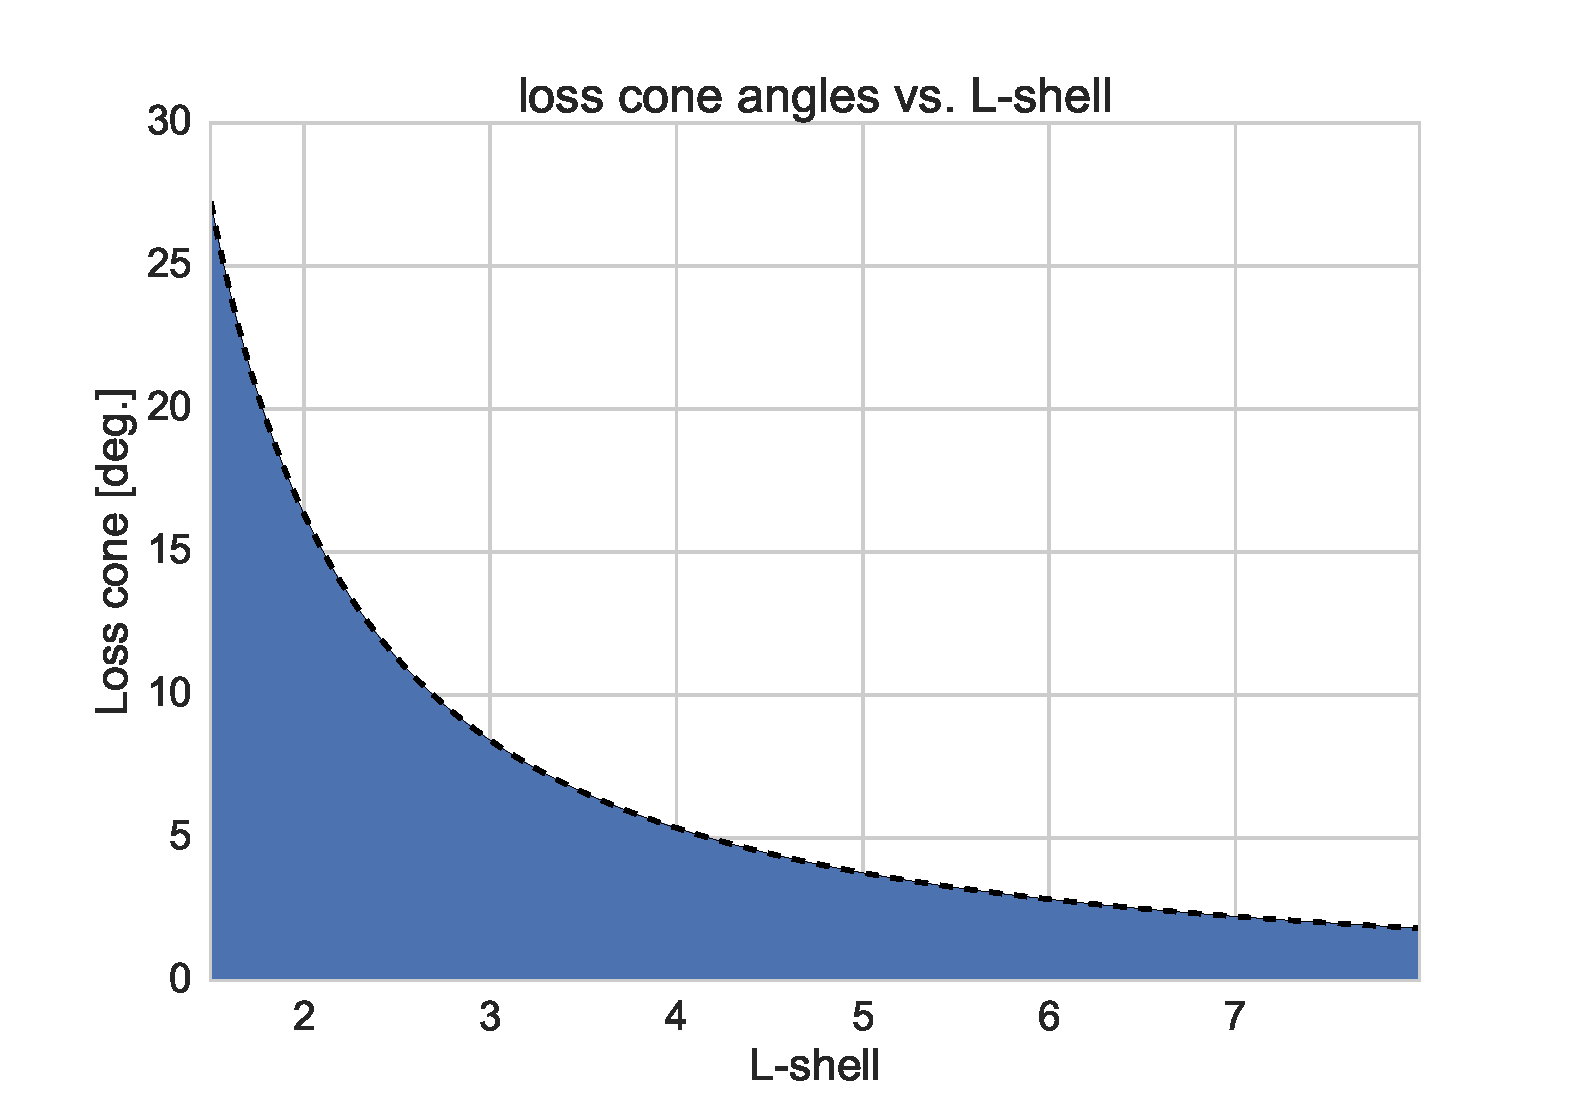
\includegraphics[width=0.8\linewidth]{gfx/lossconeangle}
	\caption{Shaded area indicates loss cone width vs. L-shell}\label{fig:losscone}
\end{figure}
Mirroring particles that are accelerated along $B$ experience an increase in $v_\parallel$ and a decrease in $\alpha_p$, increasing the likelihood the accelerated population will precipitate into the ionosphere and create aurora.
Some important L-shells for Earth are:
\begin{itemize}
	\item nightside plasmapause: 3.5 (active) to 5 (quiet)
	\item inner Van Allen Belt: 1.03 (SAA) to 3
	\item auroral oval: 4..6
\end{itemize}

\section{Auroral Energy Deposition}
The dynamic solar wind drives variability in planetary aurora at Venus \citep{phillips1986,gerard2008}, Earth, Mars \citep{bisikalo2017}, Jupiter, Saturn \citep{kivelson2005}, Uranus and Neptune \citep{arridge2015}.
Aurora at the Galilean moons are primarily driven by the Jovian magnetosphere \citep{lavrukhin2015,roth2016}.
Given the vast differences in scale, distance from the sun and plasma densities and composition, the processes in the auroral lifecycle are distinct for each planetary body.
At Earth, although some particles from the solar wind stream into the dayside geomagnetic cusp, this dissertation focuses on structured nightside aurora that is indirectly related to the solar wind loading of the magnetosphere.

The largest source of energy driving ionospheric variability at Earth is the solar wind.
The solar wind flux is filtered and stored in the magnetotail through heterogeneous and highly time-varying magnetospheric interfaces and regions.
Studies of finely structured aurora begin with data inversion from radar and optical sensors to build understanding of the auroral acceleration region dynamics. 
\textit{In situ} measurements from dense networks of on-orbit magnetometers such as ANDESITE \citep{parham2016} reveal fine current structure in the upper ionosphere.
On-orbit particle detectors such as FAST and DMSP as well as rocket borne particle detectors have been fundamental to confirming and updating theory for over 50 years.
An ultimate goal of geospace studies is to understand Earth's interaction with the solar wind as an entire system with an energy budget across scales and regions.
An ensemble of instruments study the geospace system regions at various scales. 
This dissertation examines auroral microstructure to reveal the acceleration mechanism driving the aurora.
The results may be used in the future to understand fine current structures at other planetary bodies via theory enhancement and may guide development of future instruments for use on Earth and beyond.

The solar wind peak input flux to the Earth's magnetosphere can exceed $\unit[10^{12}]{W}$ \citep{akasofu1980}.
Intense auroral precipitation of over $\nicefrac{1}{4}$ terawatt and Joule heating of several terawatts result in a diverse set of ionospheric responses \citep{lu2016}.
Given the complicated nature of energy coupling from the heliosphere through the interfaces and regions leading to dissipation in the ionosphere, a plurality of models have evolved over the past century.
A basic model for substorm auroral energy flow is depicted in Figure~\ref{fig:auroralenergy}, with a contemporary substorm model diagram in Figure~\ref{fig:collapse}.
\begin{figure}\centering 
    %the \par is necessary after each text to make the \baselineskip take effect
    \begin{tikzpicture}[node distance=1.5cm, auto]
    
    \node (in) [startstop,text width=2cm] {Solar Wind \par};
    
    \node (tail) [process, below of=in,text width=2.5cm,yshift=-0.5cm] { Magnetotail storage \textbf{growth}\par };
    
    \node (recon) [compute,below of=tail,text width=3cm,yshift=-0.5cm] { Reconnection \textbf{expansion} \par };
    
    \node (accel) [process, below of=recon, text width=3cm,yshift=-0.5cm] {Particle acceleration \textbf{dipolarization}\par };

	\node (precip) [process, below of=accel,text width=3cm,yshift=-0.5cm] { Particle precipitation \par};
	
	\node (kinetic) [compute, below of=precip,text width=3cm] { Kinetic reaction \par};
	\node (neutral) [startstop, left of=kinetic,text width=3cm,xshift=-2.5cm] {Ionospheric particles \par};
	
	\node (end) [startstop, below of=kinetic,text width=4cm] { Emissions: Light, heat, radio  \par};
    
    \draw[arrow] (in) -- (tail);
    \draw[arrow] (tail) -- (recon);
    \draw[arrow] (recon) -- (accel);
    \draw[arrow] (accel) -- (precip);
    
    \draw[arrow] (neutral) -- (kinetic);
    \draw[arrow] (precip) -- (kinetic);
    
    \draw[arrow] (kinetic) -- (end);

    
    \end{tikzpicture}
    
    \caption{Simplified model for substorm auroral energy dissipation during southward IMF, adapted from \citet{baker1996}.}
    \label{fig:auroralenergy}
\end{figure}
\begin{figure}
	\includegraphics[width=\linewidth]{gfx/substorm-catapult}
	\caption{A substorm model based on \textit{in situ} \citep{machida2009} and optical data \citep{machida2014}.}
	\label{fig:collapse}
\end{figure}
Other important processes involved in long-term evolution of aurora due to ionospheric reconfiguration include Joule heating.
Advances in observational techniques, comparative studies and increased computational power have led to refinements in these models, and this dissertation is another contribution in the observational stack.

\FloatBarrier
\subsection{Particle Loss Mechanisms}
One outcome of the loss of charged particles from the magnetosphere is the production of aurora. 
A primary driver of the finely structured aurora is substorms \citep{fukushima1962,akasofu1964,elphin1996}.
The substorm expansion phase is thought to be driven by reconnection, which is a rapid reconfiguration of open and closed field lines due to their close encounter.
During the expansion phase, a large amount of charged particles and waves are launched toward Earth.
The magnetotail plasma on the far side of the reconnection site known as a plasmoid permanently disconnects from the magnetosphere and drifts anti-sunward from Earth into the solar system. 

Substorms create an impulsive earthward restoration of the magnetotail with some of the energy carried by the Alfvén waves discussed in section \ref{sec:alfven}. 
Quantifying the energy deposition versus ionospheric altitude of precipitating electrons is central to the data inversion of this dissertation in chapters \ref{chapter:sim} and \ref{chapter:fusion}. 
Following \citet{rees1989}, we use the laboratory results of \citet{barrett1976} valid for 300..\unit[5000]{eV} that used the apparatus in Figure~\ref{fig:BellJar} to obtain
\begin{equation}\label{eq:empiricalRange}
R_{\textrm{e}^-} = 4.30 + 53.6\phi^{1.67}_{E_i}  \quad \textrm{ kg-m$^{-2}$} 
%\marginnote{e\textsuperscript- mass distance in N$_2$}
\end{equation} %Barrett & Hays p. 748
%\fxnote{Dropping the last term brings error to $10^{-8}$ from $10^{-3}$}
%\citep{JLSrs2005}  $R_{e^-} = 4.3 + 53.6K_i^{1.67} - -0.038K_i^{-0.7} \textrm{ kg-m$^2$}$} matches within 1-e3
the electron mass distance in N$_2$. 
Figure~\ref{fig:empR} shows \eqref{eq:empiricalRange}  extrapolated to energies observed at ionospheric altitudes instead of using the more complicated first principles transport equations. %paragraph 9
\begin{figure}\centering
    \includegraphics[width=0.8\textwidth,trim=30 10 30 20,clip]{gfx/JLSkamalabadiEqn2.eps}
    \caption{Mass-range according to \citet{semeter2005}}\label{fig:empR}
\end{figure}
The electron scattering depth for altitude $z$ is
\begin{equation}\label{eq:satm}
s_{\textrm{atm}} = \sec{\left( \theta_B \right)}\int_z^\infty \rho(z)\textrm{d}z \quad \textrm{ kg-m$^{-2}$} 
%\marginnote{e\textsuperscript- scattering depth}
\end{equation}
\citep{semeter2005}, where $\rho(z)$ is the mass density as obtained from the MSIS model. 

The maximum mass distance of the electron is $R_{\textrm{e}^-} = \pm 1$. The range $1 \leq R_{\textrm{e}^-} < 0$ accounts for backscattered electrons reflected back up toward the magnetosphere. 
An electron that travels mass distance $\Delta(s/R)$ loses $\Delta(E/\phi_{E_i})$ fraction of the initial energy. 
In the limit as $\Delta(s/R) \rightarrow 0$, the energy dissipation function
\begin{equation}\label{eq:energyDissFunc}
\Lambda = \frac{\mathrm{d}E/\phi_{E_i} }{ \mathrm{d}s/R }
\end{equation}
is defined \citep{semeter2005}. 
The energy dissipation function 
\begin{equation}\label{eq:qioniz}
q\left( z,\phi_{E_i} \right) = F \phi_{E_i} \Lambda \frac{\rho(z)}{R_{\textrm{e}^-}} \frac{1}{\Delta\varepsilon_{\textrm{ion}}}
\end{equation}
forms the core of the total ionization rate due to a precipitating electron beam \citep{rees1989}.
The average $\Delta\varepsilon_{\textrm{ion}}$ is typically taken \citep{semeter2005} to be \unit[35.5]{eV}.

We are interested in the contribution to $q$ of the differential flux $\Delta F$ impinging on the ionosphere with uniformly distributed energy range $\phi_{E_i} + \Delta\phi_{E_i}$. 
This is expressed in differential form \citep{semeter2005} 
\begin{equation}\label{eq:FredKernEner}
q\left( z,\phi_{E_i} \right) = \int_{\phi_{E_i}}^{\phi_{E_i}+\Delta\phi_{E_i}} \left[ \frac{\Lambda\rho\phi_{E_i} }{ \Delta\varepsilon_{\textrm{ion}} R } \right] \mathrm{d}\phi(E_i)d\phi
\end{equation}
where $\Delta F$ is represented by $\phi(E_i)\mathrm{d}E_i$. 
The differential system solution is aided by representing~\eqref{eq:FredKernEner} using the FIEFK
\begin{equation}\label{eq:JLSfiefk}
q(z) = \int_{E_{i,\textrm{min}}}^{E_{i,\textrm{max}}} A(z,E_i)\phi(E_i)\textrm{d}E_i
\end{equation}
where $A$ encompasses the energy deposition terms. 
The input differential number flux over all pitch angles $\phi(E_i)$ is the quantity estimated by the HiST system as described in chapter~\ref{chapter:sim}. 

%TODO $\phi$ is flux, not energy. Be sure it's consistent here.

\FloatBarrier
\subsection{Kinetic Reaction Outcomes}
A substantial fraction of the electrons precipitating from the magnetosphere into the ionosphere react kinetically with ionospheric particles in the \unit[90]{km} to \unit[500]{km} altitude range.
The electron precipitation flux incident on the top of the ionosphere as a function of energy $E$ is denoted as $\phi_{\mathrm{top}}(E)$ \citep{rees1989}.
A substantial fraction of the incident energy is reflected back to the magnetosphere according to the ionospheric albedo.
Albedo is equivalent to the reflection coefficient of a mismatched transmission line between the magnetosphere and ionosphere.
Secondary electrons produced by impact ionization in the ionosphere can reflect back into the magnetosphere.
This secondary electron population mirrors into the outer plasma with flux sufficient to heat the outer plasmasphere and hence significantly influence the conjugate ionospheric state \citep{khazanov2014}.
The kinetic reaction outcomes most relevant to ionospheric microscale features include unstable wave growth, ionospheric turbulence and the associated auroral microstructure.
An overview of the outcomes of ionospheric kinetic reactions are represented in Figure~\ref{fig:auroragen}, with a more detailed look at conditions favorable for auroral microstructure in Figure~\ref{fig:alfvenblock}.
\begin{figure}\centering
	\begin{tikzpicture}
	\node (precip) [startstop,text width=3cm] {Precipitation $\Phi_{top}(E)$ \par };
	
	\node (B) [process,below of=precip,yshift=-0.5cm] {$B_\parallel$ guided trajectory \par};
	
	\node (bang) [compute,below of=B,yshift=-0.25cm] {inelastic collision \par};
	
	\node (exc) [process,below of=bang,yshift=-0.5cm,text width=2cm] {excitation \unit[1..100]{eV} \par};
	\node (prompt)[process,below of=exc,xshift=-1.5cm,yshift=-1cm]{prompt \par};
	\node (forb)[process,right of=prompt,xshift=2cm]{forbidden \par};
	
	%\node (diss)[process,left of=exc,xshift=-2cm]{ dissociation \par};
	\node (ioni)[process,left of=exc,xshift=-3cm,text width=2cm] { impact ionization $\sim \unit[35]{eV}$ \par};
	\node (heat)[process,right of=exc,xshift=2cm] { heat \par};
	\node (radio)[startstop,right of=heat,xshift=2cm,text width=2cm]{ radio (ELF-HF) \par};
	
	\node (upflow)[startstop,below of=heat]{ion upflow \par};
	
	\node(secondary) [startstop,below of=ioni,yshift=-0.75cm,text width=2cm] {secondary electrons \par};
	
	\node (patt)[process,below of=prompt,text width=2.5cm,yshift=-0.5cm]{ atmospheric attenuation \par};
	\node (pass)[process,below of=patt,yshift=-0.5cm]{ filter: pass \par};
	
	\node (fatt)[process,below of=forb,text width=2.5cm,yshift=-0.5cm]{ atmospheric attenuation \par};
	\node (block)[process,below of=fatt,yshift=-0.5cm]{ filter: block \par};
	
	\node (chip)[startstop,below of=pass,text width=2cm,yshift=-0.25cm] {imaging chip \par};
	
	
	\draw[arrow] (precip) -- (B);
	\draw[arrow] (B) -- (bang);
	
	\draw[arrow] (bang) -- (exc);
	\draw[arrow] (bang) -- (ioni);
	%\draw[arrow] (bang) -- (diss);
	\draw[arrow] (bang) -- (heat);
	\draw[arrow] (bang) -- (radio);
	
	\draw[arrow] (ioni) --(secondary);
	
	\draw[arrow] (heat) -- (upflow);
	
	\draw[arrow] (exc) -- (prompt);
	\draw[arrow] (prompt) -- (patt);
	\draw[arrow] (patt) -- (pass);
	\draw[arrow] (pass) -- (chip);
	
	\draw[arrow] (exc) -- (forb);
	\draw[arrow] (forb) -- (fatt);
	\draw[arrow] (fatt) -- (block);
	
	\end{tikzpicture}
	\caption{Block diagram of auroral optical emissions generation and observation.
	The \texttt{filter} blocks represent emissions that are passed or blocked by HiST bandstop filtering.}
	\label{fig:auroragen}
\end{figure}


\FloatBarrier
\subsection{Radar Probing of Ionospheric Turbulence}
Two of the elementary electrostatic plasma wave modes discovered and characterized by \citet{tonks1929} \citep{hershkowitz2009} with the apparatus of Figure~\ref{fig:langmuirtube}  are the ion-acoustic wave and Langmuir (electron-acoustic) wave, with $\vect{k} \parallel \vect{B}$.
\begin{figure}
	\includegraphics[width=\linewidth]{gfx/langmuir-tube}
	\caption{Apparatus used by Langmuir in \citet{tonks1929} to characterize several ion and electron plasma waves.}
	\label{fig:langmuirtube}
\end{figure}
The dispersion relation for Langmuir waves is
\begin{equation}
\omega ^{2} = \omega _{pe}^{2}+3/2 k^{2}v_{e}^{2}
\end{equation}
where electron thermal velocity 
\begin{equation}
v_e = \sqrt{2 \frac{T_0}{m_e}}
\end{equation}
and $T_0$ is the temperature of the unperturbed cold plasma background.
If we suppose that background cold plasma density $n_0$ is small or that $k_\parallel$ is small, the typical observation of ISR plasma line frequency $\omega \sim \omega_{pe}$ is realized \citep{akbaridis}.
The dispersion relation for ion-acoustic waves is
\begin{equation}
\omega ^{2} = k^{2}{\frac{k_B(T_{e} + 3 T_{i})}{m_i}}
\end{equation}
and this gives rise to the ``ion line'' as depicted in Figure~\ref{fig:isrmorph}, from which the plasma parameters $n_e, T_e, T_i, v_i$ can be estimated by ISR \citep{swobodathesis}.

Very strong radar scattering can occur at radar frequency $\omega_0 \gg \omega_{pe}$, where plasma frequency is \citep{langmuir1928,chenbook}
\begin{equation}\label{eq:wpe}
\omega_{pe} = \sqrt{\frac{n_e e^2}{\epsilon_0 m_e}}.
\end{equation}
Although phase shift is expected for $\omega > \omega_{pe}$, a fact exploited in the use of GNSS TEC measurements \citep{coster1992}, constructive reflections from a sufficiently large power aperture radar yield a detectable signal.
Other minuscule signals detectable with ISR include meteoric smoke particles \citep{mahmoudian2017,baumann2016,hsu2011} and space debris down to \unit[3]{cm} at \unit[1000]{km} range with \unit[100]{ms} integration time \citep{nicolls2015}.
Almost as soon as PFISR was turned on, naturally enhanced ion acoustic lines (NEIALs) were observed, which \citet{michell2008} in Figure~\ref{fig:firstpfisrneials} associated with bright auroral forms.
\begin{figure}
	\includegraphics[width=\linewidth]{gfx/pfisrfirstneials}
	\caption{NEIALs and correlated optical intensity rise observed with the PFISR magnetic zenith beam in March 2006 \citep{michell2008}.}
	%Note, wavelength was not given in the paper. I know it's NOT the sum of all lines, but not sure which line. Probably 557.7 is my guess. Could find out from original P-DMSP data.
	\label{fig:firstpfisrneials} 
\end{figure}
NEIALs are the ISR observed results of Bragg scattering from plasma turbulence at 1/2 the radar wavenumber, leading to the ion line spectra of Figure~\ref{fig:isrmorph}(b,c).
NEIALs have been observed to occur over 140..\unit[1900]{km} altitude range \citep{schlatter2013}.





%Langmuir waves are electrostatic plasma waves where $\omega \sim \omega_{pe}$. 

%\citet{newman1994linear} notes that Langmuir bursts occur in ``moderately magnetized'' plasma where $\Omega_e \approx \omega_{pe}$.
%\citet{akbari2013} connected HF emissions in the 0.1..\unit[10]{MHz} range with NEIALS.





\section{Auroral Emissions}\label{sec:physicsemissions}

Given the historical record of deep red aurora observable at latitudes at least as low as $10^\circ$ \citep{silverman2008}, many nations and cultures have experienced aurora at least once a generation.
A rule of thumb for naked-eye visible aurora is the energy flux must be at least $\unit[1]{mW\, m^{-2}}$ or a volume emission rate greater than \unit[1]{kR}.
Modern semiconductor-based photoelectron-multiplying imaging chips give wide dynamic range and industry-leading single-photoelectron sensitivity, revealing detailed auroral features at intensities far below what human eyes and emulsified film can accomplish at high frame rates.
Purple aurora thought to correspond to \unit[427.8]{nm} and \unit[391.4]{nm} emissions is occasionally seen at the lower edge of auroral displays, when the viewing geometry and conditions are such that it is not overwhelmed by the far more intense \unit[557.7]{nm} and \unit[630.0]{nm} emissions.
%TODO This paper has info on cross sections
%\url{https://www.nist.gov/sites/default/files/documents/srd/jpcrd387.pdf}

The notional auroral spectrum in Figure~\ref{fig:VJaurora} shown over the wavelength span of interest is for a bright ICB III aurora.
\begin{figure}
	\includegraphics[width=\textwidth,trim=5 10 5 1,clip]{gfx/AuroralSpectrumLogVJ}
	\caption{Auroral spectrum in wavelength range of interest, from \citet{vallancejones1974}. }\label{fig:VJaurora}
\end{figure}
To reject metastable emissions with lifetime $\tau \gg\unit[1]{ms}$ that would smear out prompt auroral emissions, the DMC and HiST systems observed through Schott BG3 bandstop filters with specified performance in Figure~\ref{fig:BG3trans}. 
\begin{figure}\centering
	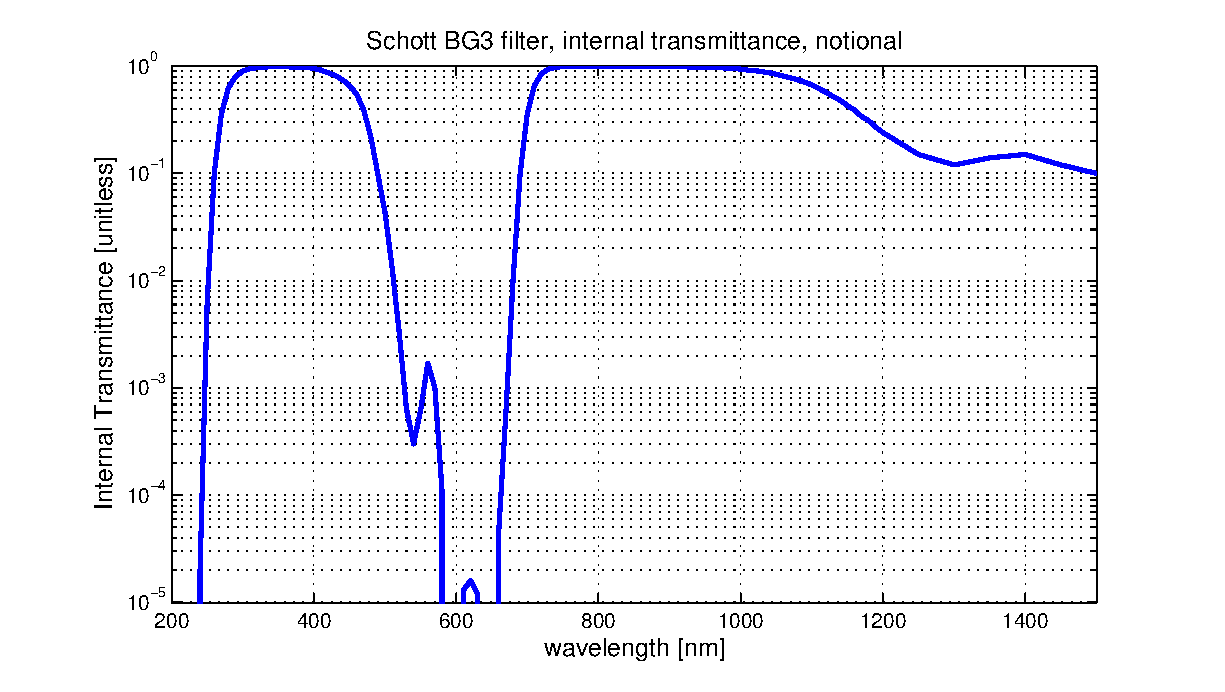
\includegraphics[width=\textwidth]{gfx/BG3transLog}
	\caption{Schott BG3 filter response}\label{fig:BG3trans}
\end{figure}
A comparison of the BG3 filter with historical and contemporary prompt emissions filters is given in Figure~\ref{fig:filters}.
The deep notch in the BG3 spectral response rejects most intense long-lifetime emissions. 
The notional EMCCD window transmission and Quantum Efficiency (QE) are shown in Figure~\ref{fig:EMCCDwindQE}.
\begin{figure}\centering
	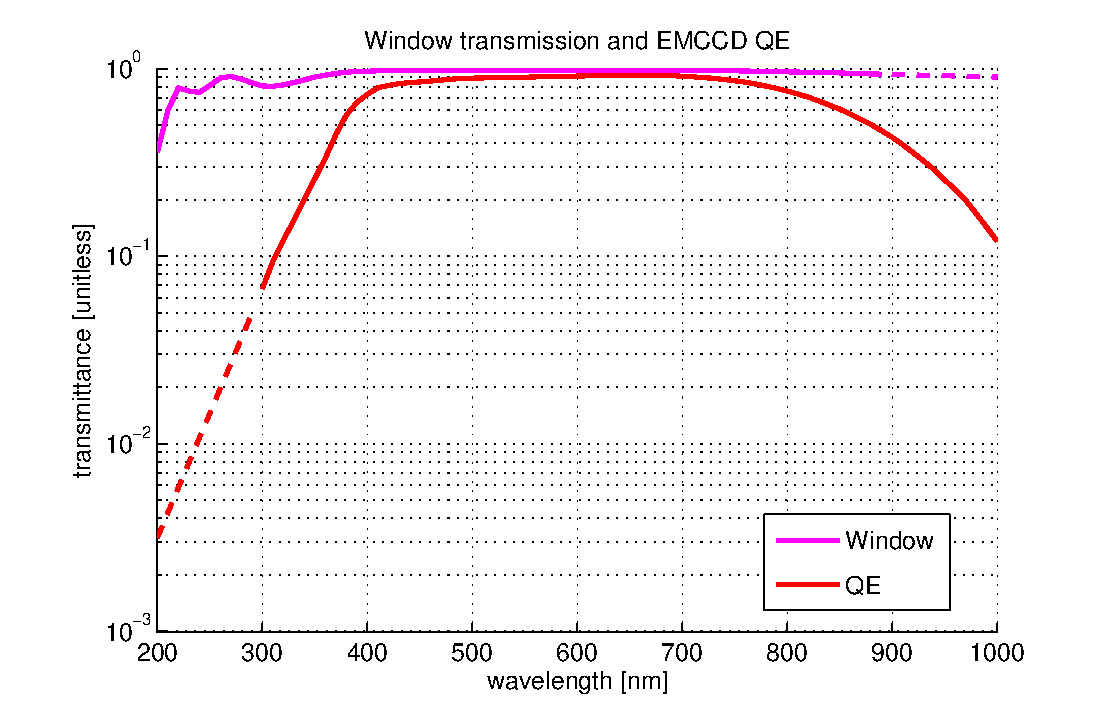
\includegraphics[width=\textwidth]{gfx/EMCCDwindowQELog}
	\caption{EMCCD window transmission and QE (extrapolated values dashed)}\label{fig:EMCCDwindQE}
\end{figure}  
The notional total system response in the wavelength range $\lambda \in [200,1000]$ nm is shown in Figure~\ref{fig:systemSpectralResp}.
\begin{figure}\centering
	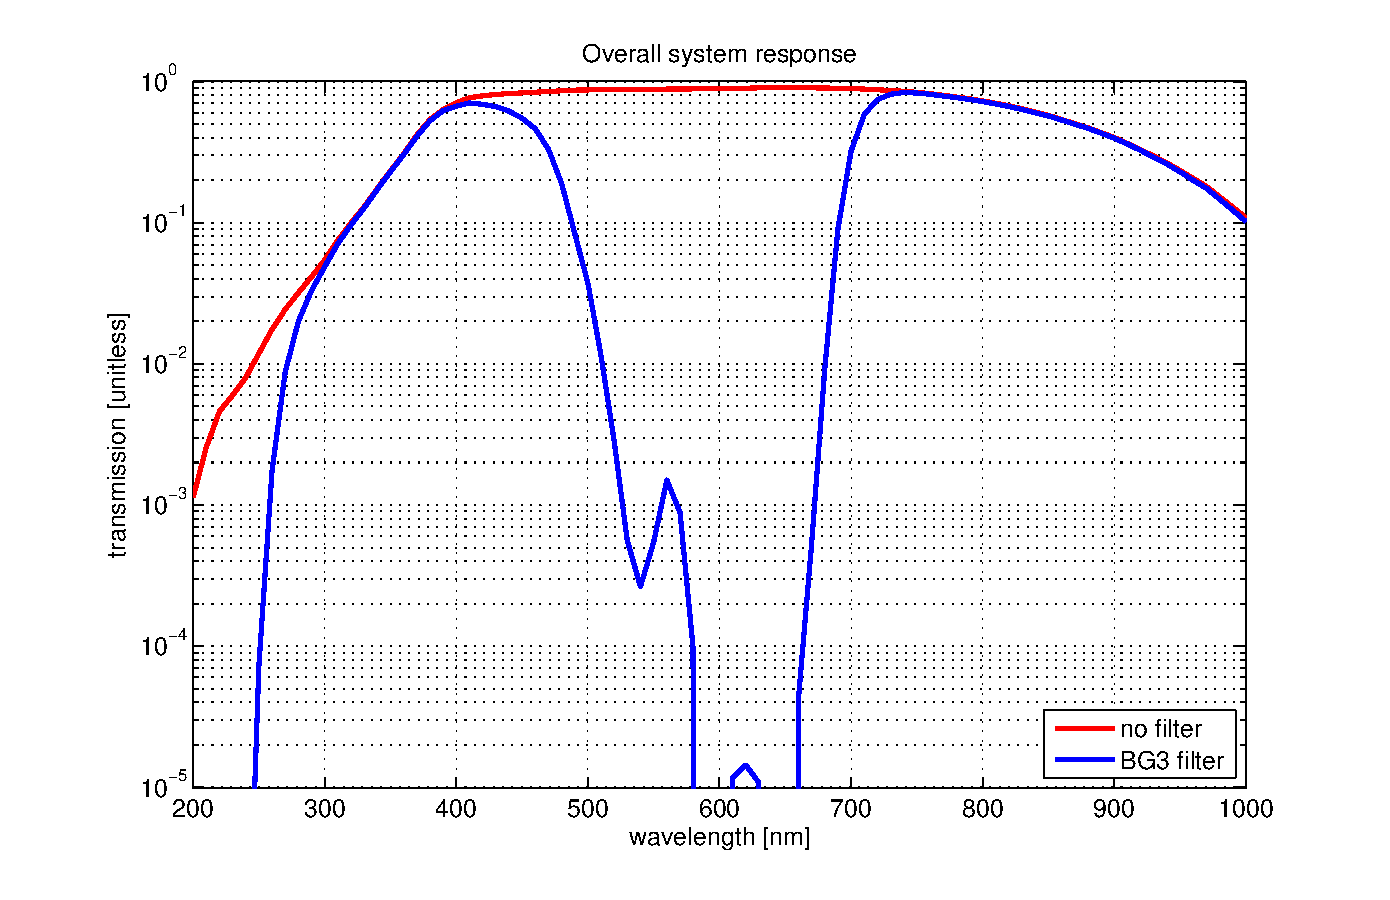
\includegraphics[width=\textwidth]{gfx/EMCCDoverallTlog}
	\caption{Overall optical transmission from lens through EMCCD chip}\label{fig:systemSpectralResp}
\end{figure}
The overall HiST transmission including atmospheric absorption, particularly significant at UV is shown in Figure~\ref{fig:optTrans}.
Several well-known auroral emission lines are given in Table~\ref{tab:spectrum} along with the optical system attenuation noted in Figure~\ref{fig:auroragen}. 

Brightness observed for the \unit[427.8]{nm} line, often taken as a proxy for high-energy precipitation has been given in the \unit[0.1..3]{kR} range \citep{dashkevich2006}.
% below 150km, dissociative recombination becomes important
Typical parameters for auroral flux as given by \citet{sandholtbook} are in Table~\ref{tab:typaurora}.
\begin{table}\centering
	\caption{Notional auroral emissions characteristics~\citep{sandholtbook}.}
    \label{tab:typaurora}
	\begin{tabular}{clll}
        \toprule
		wavelength [nm] & state & excitation energy [eV] & peak alt. [km] \\
		\midrule
		630.0 & [O] ($^1$D) & $\sim5.6$ & 200 \\
		557.7 & [O] ($^1$S) & $\sim10$ & 120 \\
		427.8 & N2$^+$ 1N & $\sim 100$ & 100 \\
        \bottomrule
	\end{tabular}
\end{table}
A starting point for the notional particle flux is typically of order $\unit[10^{13}]{m^{-2}s^{-1}}$ with energy flux of order $\unit[10]{mW \,m^{-2}}$.
A classic technique for estimating characteristic intensity $E_0$ looking up the magnetic zenith flux tube is based on the intensity ratio of line spectra.
From \citet{rees1974}, the typical ratio of $I_{6300}/I_{4278}$ is about 0.05..15, for $I_{6300}/I_{5577}$ the typical ratio is about 0.03..2.
However, for structured aurora these ratioing techniques fall apart (become highly inaccurate) since they completely lose validity away from magnetic zenith. 
%TODO justify this assertion!
An auroral observation system capable of observing within several degrees of magnetic zenith is necessary to quantify the differential number flux $\Phi_{top}$ driving structured aurora.
HiST is the first such system capable of estimating auroral precipitation characteristics with \unit[20]{ms} cadence, a rate compatible with the fastest ISR measurements as described in chapter~\ref{chapter:fusion}.

	

\section{Small scale auroral features and Alfvén waves}
Starting in the 1950s and 1960s, auroral morphology from the polar regions and auroral oval down to the mid latitudes \citep{akasofu1963} was rigorously studied.
The discovery of the magnetosphere and early understanding of its processes and regions by the mid-1960s hastened the instrument development cycle, both space- and ground-based.
Descriptions of auroral morphology depend strongly on the viewing perspective due to~\eqref{eq:bint}.
The viewer directly beneath the aurora of Figure~\ref{fig:chernouss6}(a) sees ribbons of aurora while the viewer roughly \unit[100]{km} away sees auroral curtains in Figure~\ref{fig:chernouss6}(b)--despite looking at the same section of aurora.
To motivate the disentangling of this difficult observational problem in chapter~\ref{chapter:sim}, a discussion of the processes driving microscale aurora is in order.

Despite the highly complex and time-varying linkages and paucity of coördinated \textit{in situ} measurements, a first step in understanding a ``black box'' system is quantifying the energy flux for the system and its components.
Cold ionospheric plasma, mirroring particles, the plasma sheet and direct injection from the solar wind are among  ultimate sources of precipitating particles driving the aurora.
Particle momentum carries particles across the solar system, with shocks and pickup ions redirecting the guiding center trajectory.
The structure of structured aurora is oriented along the $B_\perp$ dimension due to the frozen-in condition of plasma causing the guiding center of particles to follow geomagnetic field lines.
Structured aurora is a projection of acceleration structures in the 3000..\unit[10000]{km} altitude range.
When discussing the atmosphere, ionosphere and magnetosphere, altitude is given above mean sea level.
The finest ground-observable structures are of order \unit[10..100]{m} from even filamental electron beams due to diffusion in the ionospheric column traversed \citep{borovsky1993}.

Throughout this dissertation, ``ion'' is synonymous with a particle of positive charge. Some of the important species in the ionosphere include N$_2$, O, and N$_2^+$. 
While solar radiation throughout the ultraviolet (UV) range is responsible \citep{rees1989} for creating much of the plasma in the ionosphere, accelerated electrons are the primary driver of the aurora. 
Assumptions used in the analysis include:
\begin{enumerate}
    \item Precipitating electron energies $E > \unit[100]{eV}$
    \item Average energy loss per ionization is \unit[35.5]{eV}
    \item Excitation requires energy \unit[1..100]{eV}
%    \item \citep{semeter2005} %paragraph 17
\end{enumerate}
``Cold'' ionospheric plasma has energies of a few eV, much less than the 35~eV needed to emit a photon.
Solar wind particles have energies of order \unit[100]{eV} \citep{mottez2015}.
Only about 1\% of the $1.3 \times 10^{13}$~W flux intercepting Earth's magnetosphere is captured into the magnetosphere system \citep{mottez2015}.
Most of the intercepted flux is stored in the magnetotail, which explosively discharges every several hours in substorms, taking a few hours to restore the magnetosphere to a relaxed state, which is already recharging with solar wind flux for the next cycle.
The shear forces and turbulence in general associated with reconfiguration in any magnetic system must be communicated to other portions of the magnetoplasma.
Alfvén waves are a key mechanism for releasing stress in dynamic magnetoplasma systems.

\FloatBarrier
\subsection{Alfvén Waves}\label{sec:alfven}
Plasmas infused with magnetic field $B$ are subject to perturbations that send energy across vast distances.
On intergalactic scales, Alfvén waves have been thought to have a possible role in the evolution of cosmic rays \citep{matsukiyo2009}.
In the solar wind, theory and modeling have shown a possible role in instabilities leading to filamentation of Alfvén waves and corresponding perturbations in plasma density and $B$ \citep{kuo1988}.
In the geomagnetic system, stresses and reconfigurations from geomagnetic storms and substorms are communicated with speeds reaching to order $0.1c$. 
Alfvén waves communicate information about the constantly reconfiguring geomagnetic system across scales and great distances.

In general Alfvén waves may propagate obliquely to $B$, but for observable outcomes of electron acceleration by Alfvén waves, we assume that the Alfvén wave electric field is oriented approximately parallel to $B$.
The fingerprints of Alfvénic aurora due to Alfvén wave electron acceleration may be seen in measurements back at least to the 1970s.
The theory and modeling were solidified in the 2000s by works such as \citet{stasiewicz2000,chaston2003,chaston2007how}.
Although large fluxes of Alfvén wave-accelerated electrons in the \unit[1..10000]{eV} range are responsible for many dramatic structured auroral displays \citep{chaston2003}, numerous other methods of auroral acceleration exist \citep{borovsky1993}.

Waves in media may have fields oriented longitudinally, transverse, or oblique to the direction of propagation $\hat{k}$. 
Longitudinal waves are also known as \textit{compression} waves and transverse waves are also known as \textit{shear} waves.
Alfvén waves can reflect off the ionosphere and plasma sheet in the magnetotail repeatedly. 
Instabilities generated in ionospheric plasma by Alfvén waves have been shown by observation and modeling to be a plausible candidate for ion upflow \citep{chaston2004}, without directly involving heating \citep{zett2007,zett2008}.
Subsets of IAW such as solitary IAW and dissipative nonlinear IAW have been proposed as consistent with narrow auroral features \citep{wu2004}.
Alfvén waves have been shown to be a primary driver of dynamic aurora via \textit{in situ} observations including DMSP and FAST measurements compiled over several years.
As recounted in \citet{stasiewicz2000}, Hannes Alfvén's development and the observational confirmation of Alfvén wave theory parallels that of J. C. Maxwell's elucidation of electromagnetism.
Distinguishing between intra-Alfvénic and non-Alfvénic wave electron acceleration, essential to the $B_\perp$ structure of kinetic plasma behavior, is enhanced by the equipment described in chapter~\ref{chapter:inst} and analysis in chapters~\ref{chapter:sim} and~\ref{chapter:fusion}.

The electron thermal velocity is
\begin{equation}
v_{te} = \sqrt{2\frac{T_e}{m_e}}
\end{equation}
while Alfvén waves propagate with Alfvén velocity
\begin{equation}
v_A = \frac{B_0}{\sqrt{\mu_0\rho}}
\end{equation}
and Alfvén wave frequency
\begin{equation}
\omega = k_\parallel v_A
\end{equation}
where $v_A \ll c$ in many geomagnetic plasmas, $T_e$ is electron temperature, $m_e$ is the electron mass, $\rho=n_im_i$ is the mass density, $B_0$ is the local geomagnetic field strength and $\mu_0$ is the vacuum permeability \citep{stasiewicz2000}.
As $v_A \Rightarrow c$, the Alfvén wave behaves increasingly as if in a non-magnetized medium.
The rules of phase reversal upon reflection are the same for Alfvén waves as for general TEM waves.
Two Alfvén wave regimes referred to collectively as dispersive Alfvén waves (DAW) are described in Table~\ref{tab:alfven} and section~\ref{sec:alfvenaccel}.
\begin{table}\centering
	\caption{Dispersive Alfvén wave types relevant to auroral acceleration \citep{stasiewicz2000}.}
    \label{tab:alfven}
	\begin{tabular}{ccccc}
        \toprule
		Alfvén wave type & frequency & speed & pressure & altitude [km] \\
		\midrule
		inertial & $\omega < \omega_{ci}$  & $v_A > v_{te} $  & $ \beta < \frac{m_e}{m_i} $ & 3,000..20,000 \\ % Staciewicz 2001 pg. 429
		kinetic & & $v_A < v_{te}$ & $\frac{m_e}{m_i} < \beta < 1$ & $\gtrsim 20,000$ \\
        \bottomrule
	\end{tabular}
\end{table}


\FloatBarrier
\subsection{Alfvénic Auroral Acceleration}\label{sec:alfvenaccel}
Electron-driven aurora can most broadly be categorized as diffuse or discrete \citep{newell2009}.
Diffuse and structured auroral arcs driven by inverted-V potential structures may be time-modulated in flux by ion-acoustic resonances.
Regions with sharp potential gradients are included in the category of inverted-V precipitation driven aurora, along with the smoothly varying potential structure the name implies \citep{newell2009}.
Inverted-V arcs may translate, but they do not experience splitting or flaming behavior, and NEIALs are not associated with them.
The diffuse aurora life cycle is dominated by resonant wave-particle interactions scattering plasma sheet electrons in the loss cone \citep{Ni2016}.
Time-modulated diffuse aurora is driven by mechanisms with little dispersion relative to discrete auroral drivers.
\begin{figure}\centering
	\begin{tikzpicture}
	\node (mirror) [startstop] {Mirroring ions and electrons \par };
	
	\node (fac) [process,below of=mirror,xshift=-3cm,yshift=-0.5cm] {FAC \par};
	
	\node (ion) [startstop,below of = fac,text width=3cm,yshift=-0.5cm] {ion/electron diffuse aurora \par};
	
	\node (inv) [process,right of = fac,xshift=4cm] { Inverted-V, double layer \par};
	
	\node (mono) [startstop,below of = inv,text width=4cm,yshift=-0.5cm] { Discrete, monoenergetic aurora \par };
	
	
	\draw[arrow] (mirror) -- (fac);
	\draw[arrow] (fac) -- (ion);
	
	\draw[arrow] (mirror) -- (inv);
	\draw[arrow] (inv) -- (mono);
	
	\end{tikzpicture}
	\caption{Block diagram of non-Alfvénic aurora acceleration mechanism.}
	\label{fig:nonalfvenblock}
\end{figure}

\citet{chaston2007how,mcfadden1999} note that particle acceleration relevant to ground-observable aurora occurs along $B_\parallel$ and occurs in altitude ranges from about 3000..\unit[20000]{km}.
\citet{stasiewicz2000} cited Freja measurements showing that while cold plasma $\sim \unit[5]{eV}$ heavily dominates from 1000..8000~km in the auroral zone and polar cap, in Alfvénic turbulence regions almost no cold electrons exist.
The source of sudden large flux of low energy electrons is thought to come from Alfvén wave acceleration of mirroring electrons into the loss cone.
Alfvén waves operate across a wide range of regimes from accelerating relativistic particles in galaxy clusters \citep{brunetti2004} to the Earth's lower magnetosphere.

%To describe the nature of Alfvén waves responsible for auroral acceleration, we begin with Ohm's Law
%\begin{equation}
%\vect{j} = \sigma \vect{E}
%\end{equation}
%that becomes modified in the plasma surrounding Earth due to the collisionless nature of plasma above the lower ionosphere.
%The magnetohydrodynamic momentum balance equation
%\begin{equation}\label{eq:mhdmomentum}
%\rho \frac{\textrm{d}\vect{v}}{\textrm{d}t} = \rho \left(\frac{\partial\vect{v}}{\partial t} + \vect{v} \cdot \nabla \vect{v}\right) = \vect{j} \times \vect{B} - \nabla p
%\end{equation}
%for ions and electrons are subtracted to obtains the Generalized Ohm's Law \citep{paschmann2003}
%\begin{equation}
%\vect{E}+\vect{v}\times\vect{B} = \eta \vect{j} + \frac{1}{ne}\left(\vect{j} \times \vect{B} - \nabla \cdot p_e\right) + \frac{m_e}{ne^2}\left(\frac{\partial \vect{j}}{\partial t} + \nabla \cdot \left(\vect{j}\vect{v} + \vect{v}\vect{j}\right)\right)
%\end{equation}

An important scale concerning Alfvén waves is the electron inertial length or skin depth \citep{paschmann2003}
\begin{equation}\label{eq:einert}
\lambda_e = c/\omega_{pe}
\end{equation}
which relates to ion inertial length
\begin{equation}
\lambda_i = \lambda_e \left(\frac{m_e}{m_i}\right)^{-1/2}.
\end{equation}
In a notional topside ionosphere using~\eqref{eq:wpe} and~\eqref{eq:einert} and assuming $n_e = \unit[10^{10}]{m^{-3}}$
\begin{equation}
\lambda_e = c \left( \frac{n_e e^2}{\epsilon_0 m_e} \right)^{-1/2} = \unit[53]{m}
\end{equation}
which is consistent with sub-\unit[100]{m} width auroral arc features associated with Alfvénic accelerated electrons.
Another relevant scale (assuming as is usual quasistatic ions) is the Debye length \citep{langmuir1928}
\begin{equation}
\lambda _{D}={\sqrt {\frac {\varepsilon_0 k_B T_e}{n_e e^{2}}}}
\end{equation}
that in the magnetosphere is of order \unit[100]{m}.
Inertial waves are backward waves, where the direction of phase velocity is opposite the wave vector $\overrightharp{k}$.
The $\vect{E} \parallel \vect{B}$ field is supported by the electron inertia \citep{stasiewicz2000}.
The dispersion relation for inertial Alfvén waves (IAW) is \citep{stasiewicz2000}
\begin{equation}\label{eq:dispiaw}
\omega^2 = \frac{k^2_\parallel v^2_A}{1+k^2_\perp \lambda^2_e}.
\end{equation}
Using the definition of group velocity we obtain \citep{stasiewicz2000}
\begin{equation}
\frac{\partial \omega}{\partial \vect{k}} = \widehat{z} \frac{v_A}{\sqrt{1+k^2_\perp \lambda_e^2}} - \widehat{x} \omega \lambda_e \frac{k_\perp \lambda_e}{1+k^2_\perp \lambda_e^2}
\end{equation}
which essentially says that the Alfvén wavelength increases with time along $B_\perp$ while accelerating electrons along $B_\parallel$.
The DAW propagates in a conical region with apex angle \citep{semeter2008}
\begin{equation}
\tan \theta_a = \frac{\omega}{\omega_{ci}} \sqrt{\frac{m_e}{m_i}},
\end{equation}
%In left-handed material (artificial metamaterial only) $\vect{k}$ can be opposite Poynting vector.
This cone-like structure is represented in Figure~\ref{fig:alfvencone}.
\begin{figure}
	\includegraphics[width=0.9\linewidth]{gfx/alfven_cone}
	\caption{Alfvén wave acceleration cone structure with alternating up/down acceleration \citep{semeter2008}}\label{fig:alfvencone}
\end{figure}

%\subsection{Alfvén waves in the upper magnetosphere}
%Kinetic Alfvén waves (KAW) were first measured by the Polar satellite \citep{wygant2002} to have narrow widths of order 20~km.
%This is on the order of the ion-acoustic gyroradius, which facilitates KAW particle acceleration along $B_\parallel$.
%
%\citet{lysak1996} cited an Alfvén dispersion relation that treats the KAW-IAW-electrostatic regime as a continuüm throughout the DAW acceleration lifecycle.
%
%Alfvén wave-driven pulsating aurora has also been observed \citep{fukuda2016}.
Observational cadence with high-resolution electron spectrometers was typically of order of \unit[30..50]{ms} \citep{michell2016} on rockets and satellites such as MMS.
\citet{michell2016} motivated the new millisecond sampling electron spectrometer flown aboard the 2014 GREECE rocket by noting that auroral microstructure has sub-\unit[100]{m} widths and apparent $B_\perp$ velocities of up to \unit[20]{km/s}.
Nyquist theorem requires sampling at least as fast as $100/20000/2 = \unit[2.5]{ms}$.
Figure~\ref{fig:greece-precip} shows that \unit[1]{ms} is adequate for catching numerous DAW coming in rapid succession on this flight.
\begin{figure}
	\includegraphics[width=\linewidth]{../gfx/greece-flux}
	\caption{Dispersive flux packets on GREECE rocket. \citep{michell2016}}
	\label{fig:greece-precip}
\end{figure}
The optical instrumentation described in chapter~\ref{chapter:inst} and the ISR described in chapter~\ref{chapter:fusion} are likewise of adequate sampling rate to resolve Alfvénic aurora.
A key distinction is that cameras can turn on and run indefinitely, thanks to the algorithm of chapter~\ref{chapter:discrim}, giving better chances for joint instrument observations.
Rockets and satellite provide invaluable \textit{in situ} measurements, but only for a single rapidly moving point (or cluster of points) in time.
Having rounded out the introductory theory necessary for the HiST system design, chapter~\ref{chapter:inst} describes the DMC and HiST systems, along with ISR and other instruments used in the joint ISR-optical analysis.

